\documentclass[12pt,a4paper]{article}
\usepackage[a4paper]{geometry}
\usepackage{fontenc}
\usepackage{helvet}
\usepackage{parskip}

\usepackage{fancyhdr}




\usepackage{siunitx}

\usepackage{booktabs}
\usepackage{tabu}

\usepackage[backend=bibtex]{biblatex}
\bibliography{Gas_Flow.bib}






\begin{document}
\begin{center}
    \vspace*{0.5cm}
    
    \Huge
    \textbf{Gas Flow Lab Report}
    
    \vspace{0.5cm}
    
    \normalsize
    \textbf{Haoze Pang}
    
    \textbf{1019521}
    
    \vspace{0.5cm}
    
    Department of Physics and Astronomy
    
    The University of Manchester
\end{center}
\vspace{18pt}


	\section{Introduction}
	
	 In this experiment, the researcher tries to determine the properties of Helium (He) and Argon (Ar) gas by analysing the pressure in a thin tube as gases flow through it. 
	
	The researcher divided this experiment into two parts. In the first part, the experimenter created a laminar flow environment using a long tube and determined the viscosity of both gases. 
	%The experimenter deduced several microscopic properties of He and Ar using Kinetic Theory from the viscosities of the gases. 
	In the second part of this experiment, the experimenter created a molecular flow environment in a short tube. He then determined He and Ar's pumping speed by measuring the tube's pressure.
	
	\section{Theory}
	\subsection{Laminar Flow Theory}
		Laminar flow is a type of gas flow that is steady, streamlined, and without swirls. In such a flow regime, layers of gas with varying velocities exist.  The speed of gas in the middle layer is moving fastest. The rate decreases as it moves toward the walls of the tube and reaches zero at the wall. A force is associated with this velocity gradient and is characterised by viscosity $\eta$. 
		
		Now, we introduce theories that determine viscosity.
		Poiseuille's Equation,\\
			\begin{equation}
				Q=\frac{\pi*a^4*(p_{in}^2(t)-p_{out}^2)}{16 \eta l},
				\label{Poiseuille's Equation}
			\end{equation}
		relates the viscosity of the gas, the pressure difference, the dimensions of the tube the gas flows through, and its flow rate. Here, $a$ is the radius, and $l$ is the length of the tube. $p_{in}$ is the pressure at the input end of the tube, and $p_{out}$ is the pressure at the output end of the tube. In our laminar flow experiment, $p_{out}$ is the atmospheric pressure. We also know that\\
		\begin{equation}
			Q=-V_{in} \diff{p_{in}(t)}{t}.
			\label{flow rate}
		\end{equation}
	Equating equation \ref{Poiseuille's Equation} and \ref{flow rate}, then integrating, we obtain\\
		\begin{equation}
			\ln (\frac{p_{in}(t)-p_{out}}{p_{in}(t)+p_{out}})=-\frac{\pi a^4 p_{out}}{8 \eta l V_{in}} \cdot t+C
			\label{equation: best-fit line on Laminar}
		\end{equation}	
	
	So, if we plot $\ln (\frac{p_{in}(t)-p_{out}}{p_{in}(t)+p_{out}})$ as a function of time, we can use the gradient of the best-fit line ($m$) to determine the viscosity of a gas. From equation \ref{equation: best-fit line on Laminar} can deduce that\\
	\begin{equation}
		\eta=-\frac{\pi a^4 p_{out}}{8 m l V_{in}}. 
		\label{eq: viscosity}
	\end{equation}
	\subsection{Molecular Flow Theory}
	In laminar flow, the difference in pressure between two ends of the tube is sufficiently low that gas particles move slowly. The result is that collisions mainly occur between gas molecules and the wall. Here, the rate of gas flow is proportional to the input pressure and is given by the equation\\
	\begin{equation}
		Q=S p_{in}(t). \label{eqn: Q in molecular}
	\end{equation} 
	The proportionality constant $S$ is referred to as pumping speed.
	Equating \ref{eqn: Q in molecular} with Poiseuille's Equation and integrating, we have\\
	\begin{equation}
		\ln (p_{in}(t)-p_r)=-\frac{St}{V_{in}}+C,\label{eqn: Molecular best fit}
	\end{equation}
	where $p_{in}$ is the input pressure as a function of time, $p_r$ is the residual pressure, and $V_{in}$ is the volume of gas.\cite{Lab_Instruction}
	\section{Methods}
	\subsection{Preparation}
	We set up the equipment as the figure shows.
	\begin{figure*}[h!]\label{Apparatus}
		\begin{center}
			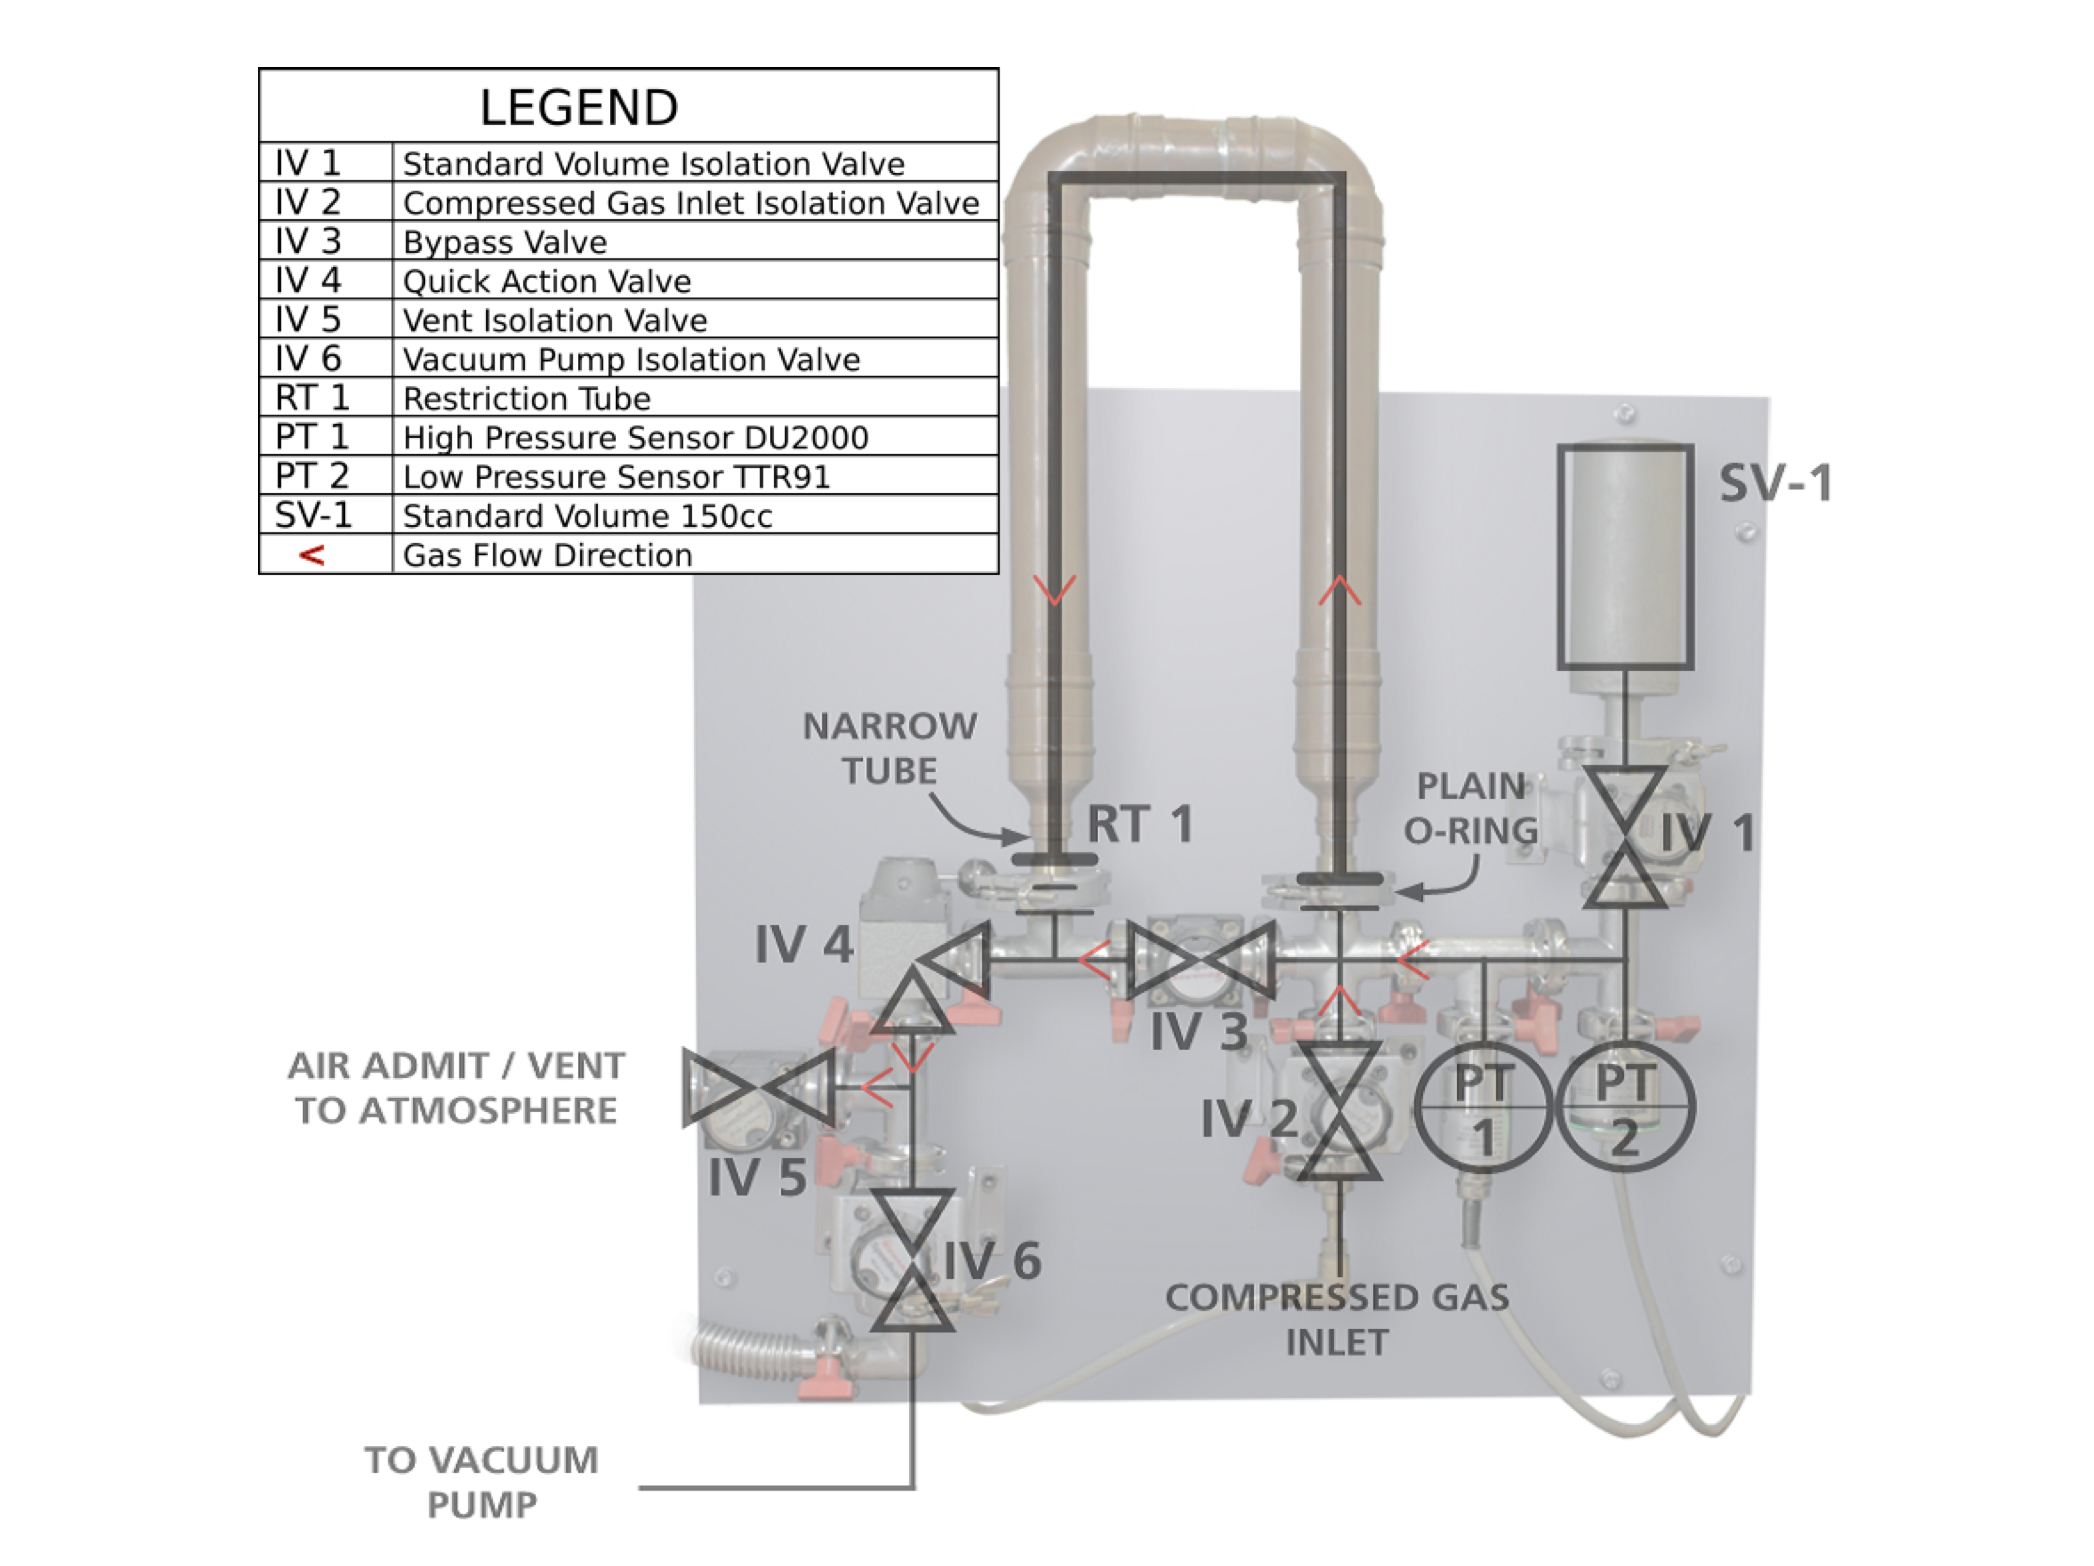
\includegraphics[scale=0.3]{Gas_Flow_apparatus.png}
			\caption{In the experiment, gas flow through a narrow tube, RT1. PT1, which has a higher range, is the gauge used in the Laminar Flow trial. PT2, which has a lower measure range, is the gauge employed in molecular flow measurement.\cite{Lab_Instruction}
}
		\end{center}
	\end{figure*}
	
	Now, we attempt to determine the input volume $V_{in}$ and atmospheric pressure, $p_0$, which corresponds to $p_{out}$ in the laminar flow experiment.
	We operated the equipment in the following order.
		%\item Close all valves.\label{item: start}
		%\item Open Quick Action Valve (IV 4) and Bypass Valve (IV 3).
		%\item Open Vacuum Pump Isolation Valve (IV 6).
		%\item Wait for the reading on PT2 to drop to a magnitude of $10^{-3}$.\\
			%The steps above aim to evacuate residual gas in our narrow tube.\\
	First, we closed all valves. Then, we opened IV 1 and IV 3. We continued to open IV 2 and pump Helium in, and as the reading on PT1 stabilises, recorded it as $p_x$. Here, we recorded $p_x$, the pressure corresponding to a volume, which is the sum of the standard valve and the input volume. We closed all valves, and opened IV 4, IV 5, and IV 3. As the reading on PT1 stabilises, we recorded it as $p_0$. Here, we measured the atmospheric pressure, which corresponds to the volume of the standard valve.  
	
	Assuming constant temperature, we have ideal gas law in the form\\
	\begin{equation*}
		p_1 \cdot V_1 = p_2 \cdot V_2
	\end{equation*}
	In this measurement,\\
	\begin{equation*}
		p_0 \cdot V_s = p_x \cdot (V_s+V_{in}),
	\end{equation*}
	where $V_s=150 \si{c\metre^3}$ is the volume of the standard valve.
	Solving the equation above, we determined, 
	$$V_{in}= 6 \times 10 ^{-4} \pm 6 \cdot 10^{-3} \si{\metre^3}.$$
	Note that in the calculation of the uncertainty on $V_{in}$, we ignored the term $V_s$ as the uncertainty on it is much smaller than the other two terms.
		
	
	\subsection{Laminar Flow}		
	In this part of the experiment, the experimenter operated the apparatus in the following order to create a laminar flow environment.
	We first placed a long tube in RT 1, then closed all valves.
	(step: Start). 
	We proceeded to open Quick Action Valve (IV 4) and Bypass Valve (IV 3), next opened Vacuum Pump Isolation Valve (IV 6). We subsequently waitted for the reading on PT2 to drop to a magnitude of $10^{-3}$. The steps above aim to evacuate any residual gas in our narrow tube.
		
	We then closed IV 6, IV 4, and IV 3, and opened IV 2 and pump Helium in. 
	(step: Pump gas)
	When the reading on PT1 reaches approximately \SI{2000}{m\bar}, we closed IV2. We started to record data at this point with a minimum interval of 0.5s.
		, then opened Vent Isolation Valve (IV5). We waited until the reading on PT1 reaches atmospheric pressure, in this particular experiment, \SI{1024}{m\bar} 
	(step: End)
	We repeated step 'Start' to 'End' twice, changed the gas in step 'Pump gas' to Ar, and repeated step 'Start' to 'End' thrice to collect data on Ar.
	\subsection{Molecular Flow}	
	In this part of the experiment, we operated the equipment in the following order to create a molecular flow environment.
	\begin{enumerate}
		\item Close all valves.
		\item Open IV 4 and IV 6
		\item Wait for the readings on PT2 to drop to a magnitude of $10^{-4}$
		\item Close IV 4
		\item Open IV 2 and pump gas in until the pressure is about $5$ to $8$ \si{m\bar}\label{Pump gas}
		\item Start to record data with minimum logging interval of  $45$\si{\second}
	\end{enumerate}
	Repeat this process but change the gas in step \ref{Pump gas} to Ar.
	\section{Calculations and Results}
	\subsection{Laminar Flow}
	The experimenter plotted $\ln (\frac{p_{in}(t)-p_{out}}{p_{in}(t)+p_{out}})$ against time $t$ and using LSFR to generate a best fit line.
			\begin{table}[h!]
			 \begin{tabu}{*{3}{X[c]}}
    			\toprule
    				Number of trials & Gradient & Reduced $\chi^2$\\
    			\midrule
       				1 & $ -2.52 \times 10^{-2} \pm 9.34 \times 10^{-4}$ & 0.01 \\ 
      				2 & $ -2.54 \times 10^{-2} \pm 1.25 \times 10^{-3}$ & 0.01  \\ 
       				3 & $ -2.52 \times 10^{-2} \pm 1.67 \times 10^{-3}$ &0.01  \\
   				 \bottomrule
    		\end{tabu}
    		\caption{This table shows the gradient ($m$) and reduced $\chi^2$ of the best-fit line of our data on He.}
		\end{table}
	
	The weighted mean on the gradient $m$ is $-2.5 \times 10^{-2} \pm 6.83 \times 10^{-4}$ \si{\second^{-1}}.		
	Checking the manufacture notes on the long tube, we obtain the following data:
	$a=0.01 \pm 0.005$ mm,  $l=30.0 \pm 0.5$ mm.
	
	Substituting values to equation \ref{eq: viscosity}, we reckon
	\begin{equation*}
		\eta_{He}= 9 \cdot 10^{-6} \pm 1.29 \cdot 10^{-2} \si{\newton\cdot\second\per\metre^2}.
	\end{equation*}
	
	Similarly, we have the data on Ar as the following:
	\begin{table}[h!]
			 \begin{tabu}{*{3}{X[c]}}
    			\toprule
    				Number of trials & Gradient & Reduced $\chi^2$\\
    			\midrule
       				1 & $ -1.68 \times 10^{-2} \pm 6.15 \times 10^{-4}$ & 0.10\\ 
      				2 & $ -1.65 \times 10^{-2} \pm 6.13 \times 10^{-3}$ & 0.09\\ 
       				3 & $ -1.64 \times 10^{-2} \pm 6.08 \times 10^{-3}$ & 0.09\\
   				 \bottomrule
    		\end{tabu}
    		\caption{This table shows the gradient ($m$) and reduced $\chi^2$ of the best-fit line of our data on Ar.}
		\end{table}
		
	The weighted mean on the gradient $m$ is $-1.65 \times 10^{-2}$ \si{\second^{-1}}. Substituting values to equation \ref{eq: viscosity}, we reckon
	\begin{equation*}
		\eta_{Ar}= 4.1 \times 10^{-5}  \si{\newton\cdot\second\per\metre^2}.
	\end{equation*}
	
	\subsection{Molecular Flow}
	Now, we calculate the pumping speed of He. We plotted $\ln(p_{in}(t)-p_r)$ against time, with a time interval of $1500\si{\second}<t<3000\si{\second}$, which we determine as the timescale where the gas glow is characterised as molecular flow.	 (Note that we calibrated our data by multiplying a different constant for other gases' original data.) Using LSFR, we generated the best fit line on the data.
	\begin{figure}[h!]
		\begin{center}
			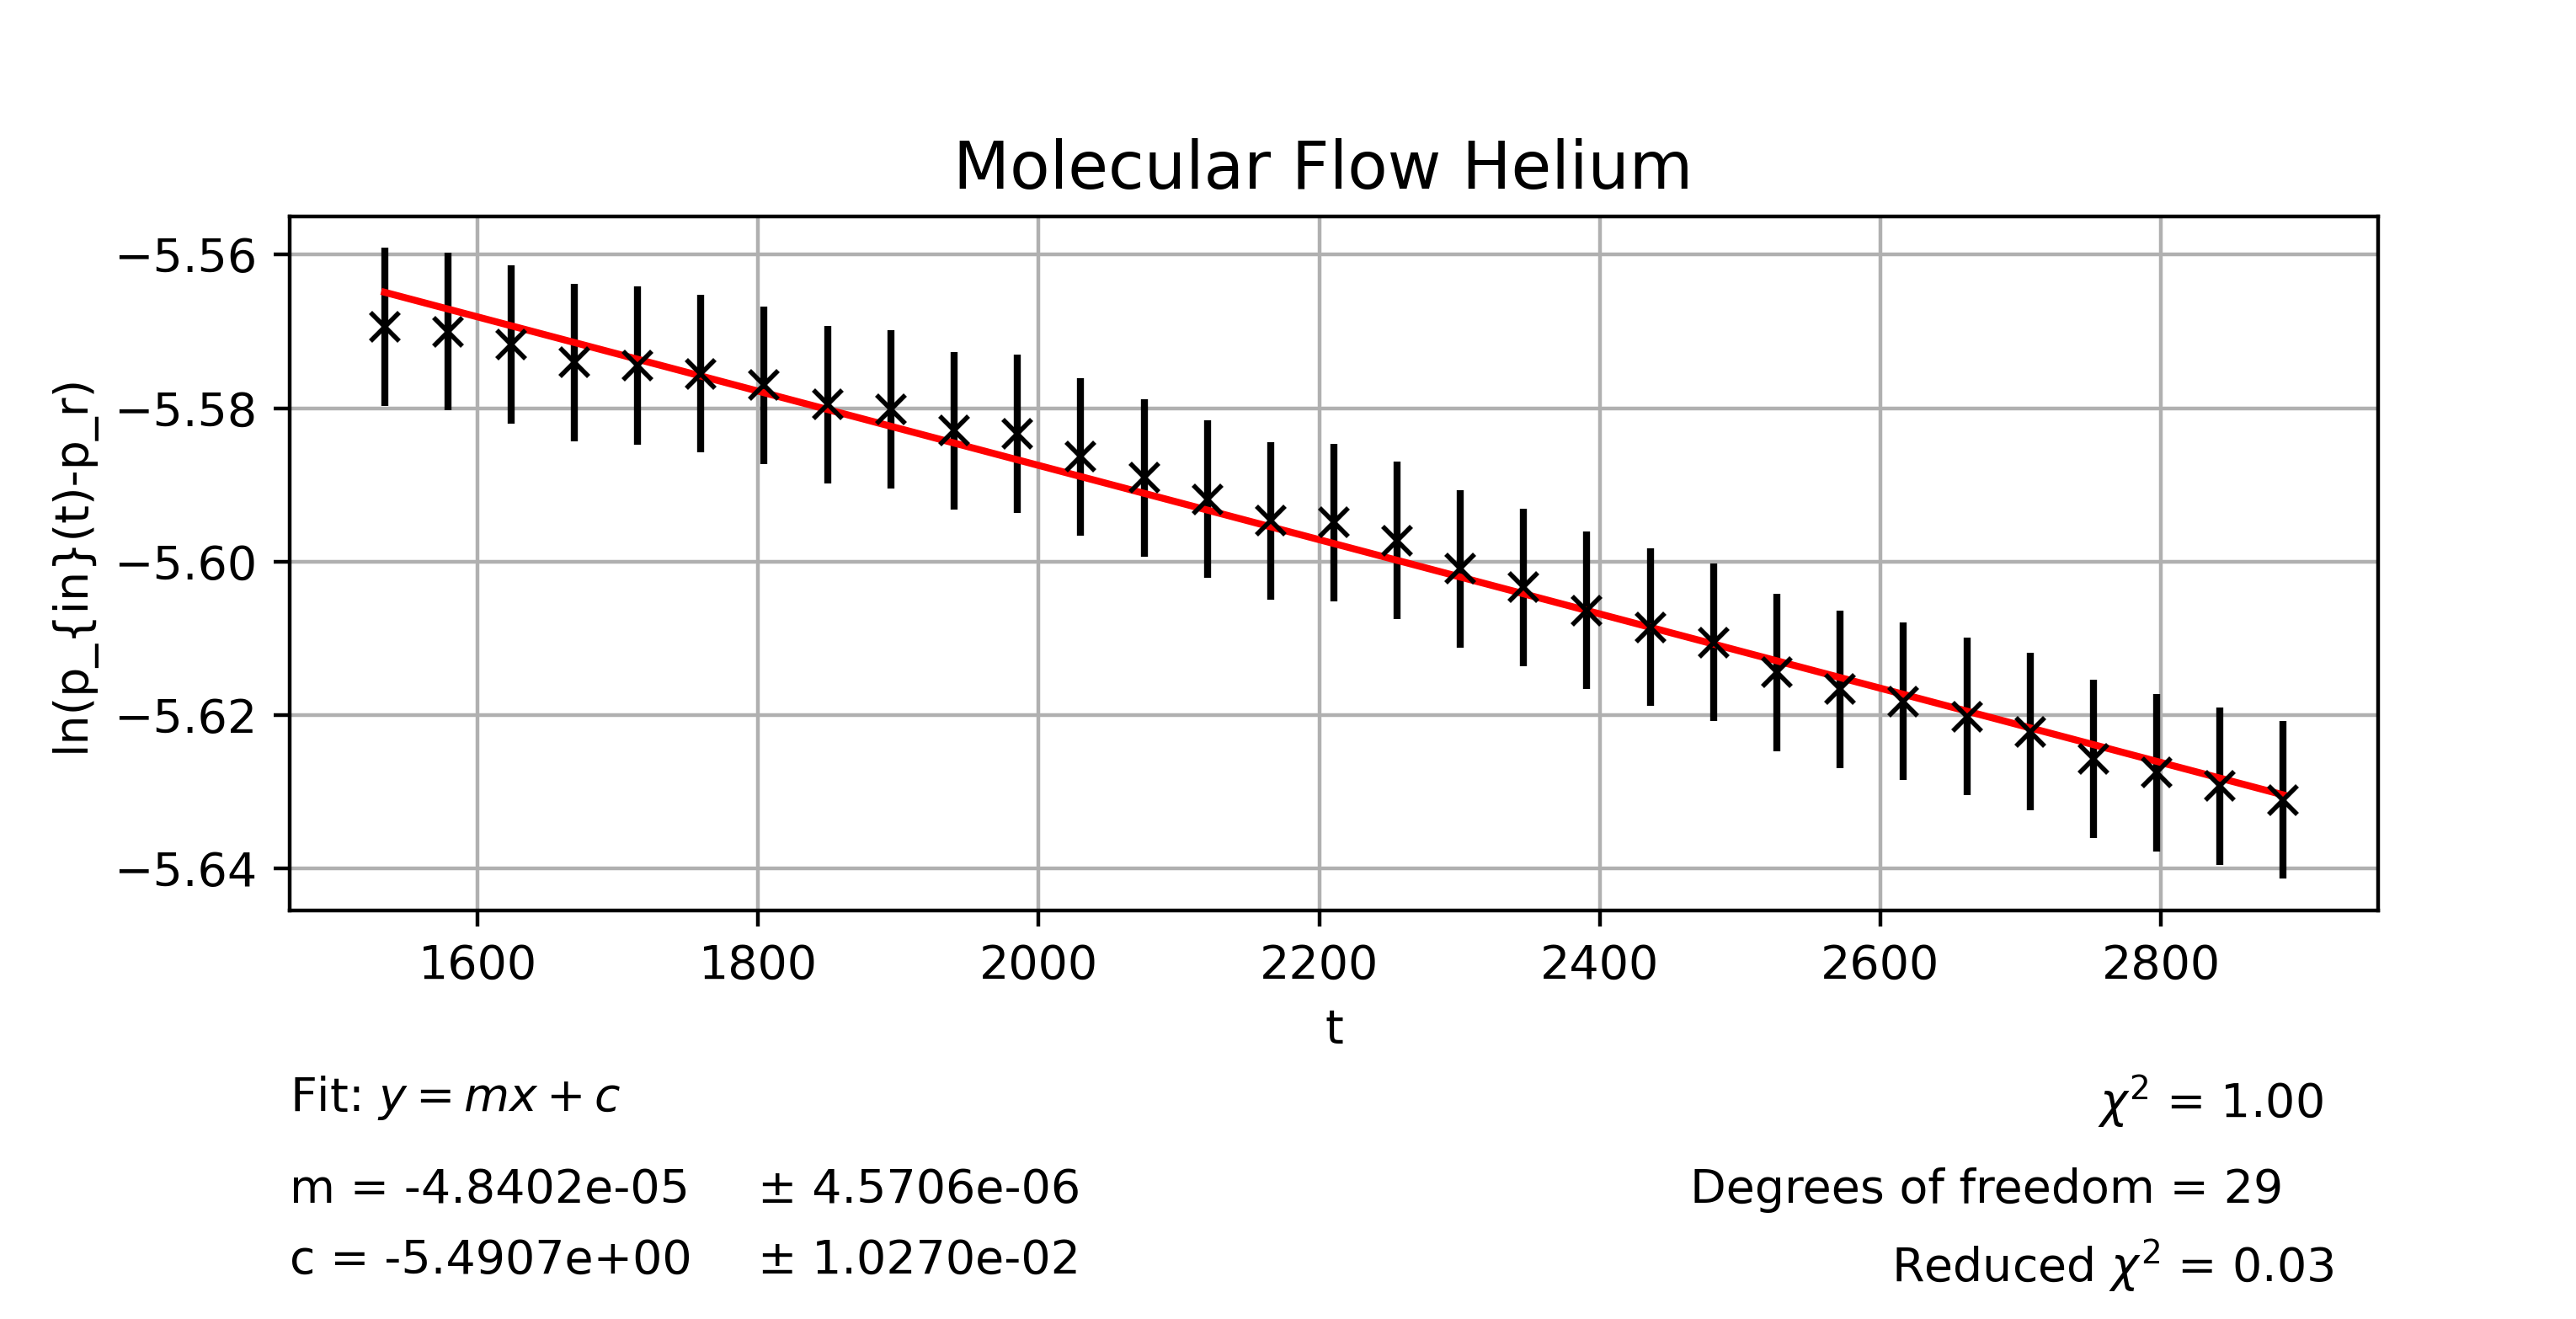
\includegraphics[scale=0.5]{Molecular_Helium_best_fit_line.png}
		\caption{This graph shows the best-fit line of our data.}
		\end{center}
			\end{figure}
 	
 	We have the gradient $m=-4.840 \time 10^{-5} \pm 4.5 \times 10^{-6}$. Also, from equation \ref{eqn: Molecular best fit}, we know that\\
 	\begin{equation}
 		S=-m V_{in}.
  	\end{equation}
  	Substituting $m$, we obtain\\ 
  	\begin{equation}
  		S_{He}= 3 \pm 10 \si{\meter^3\per\second}.
  	\end{equation}
  	
  We identified the uncertainty in $V_{in}$ as the main factor contributing to the uncertainty of $S$.\\
  
  Likewise, we now compute the pumping speed of Ar. We generated the best-fit line, this time choosing $1750\si{\second}<t<2750\si{\second}$.
  \begin{figure}[h!]
		\begin{center}
		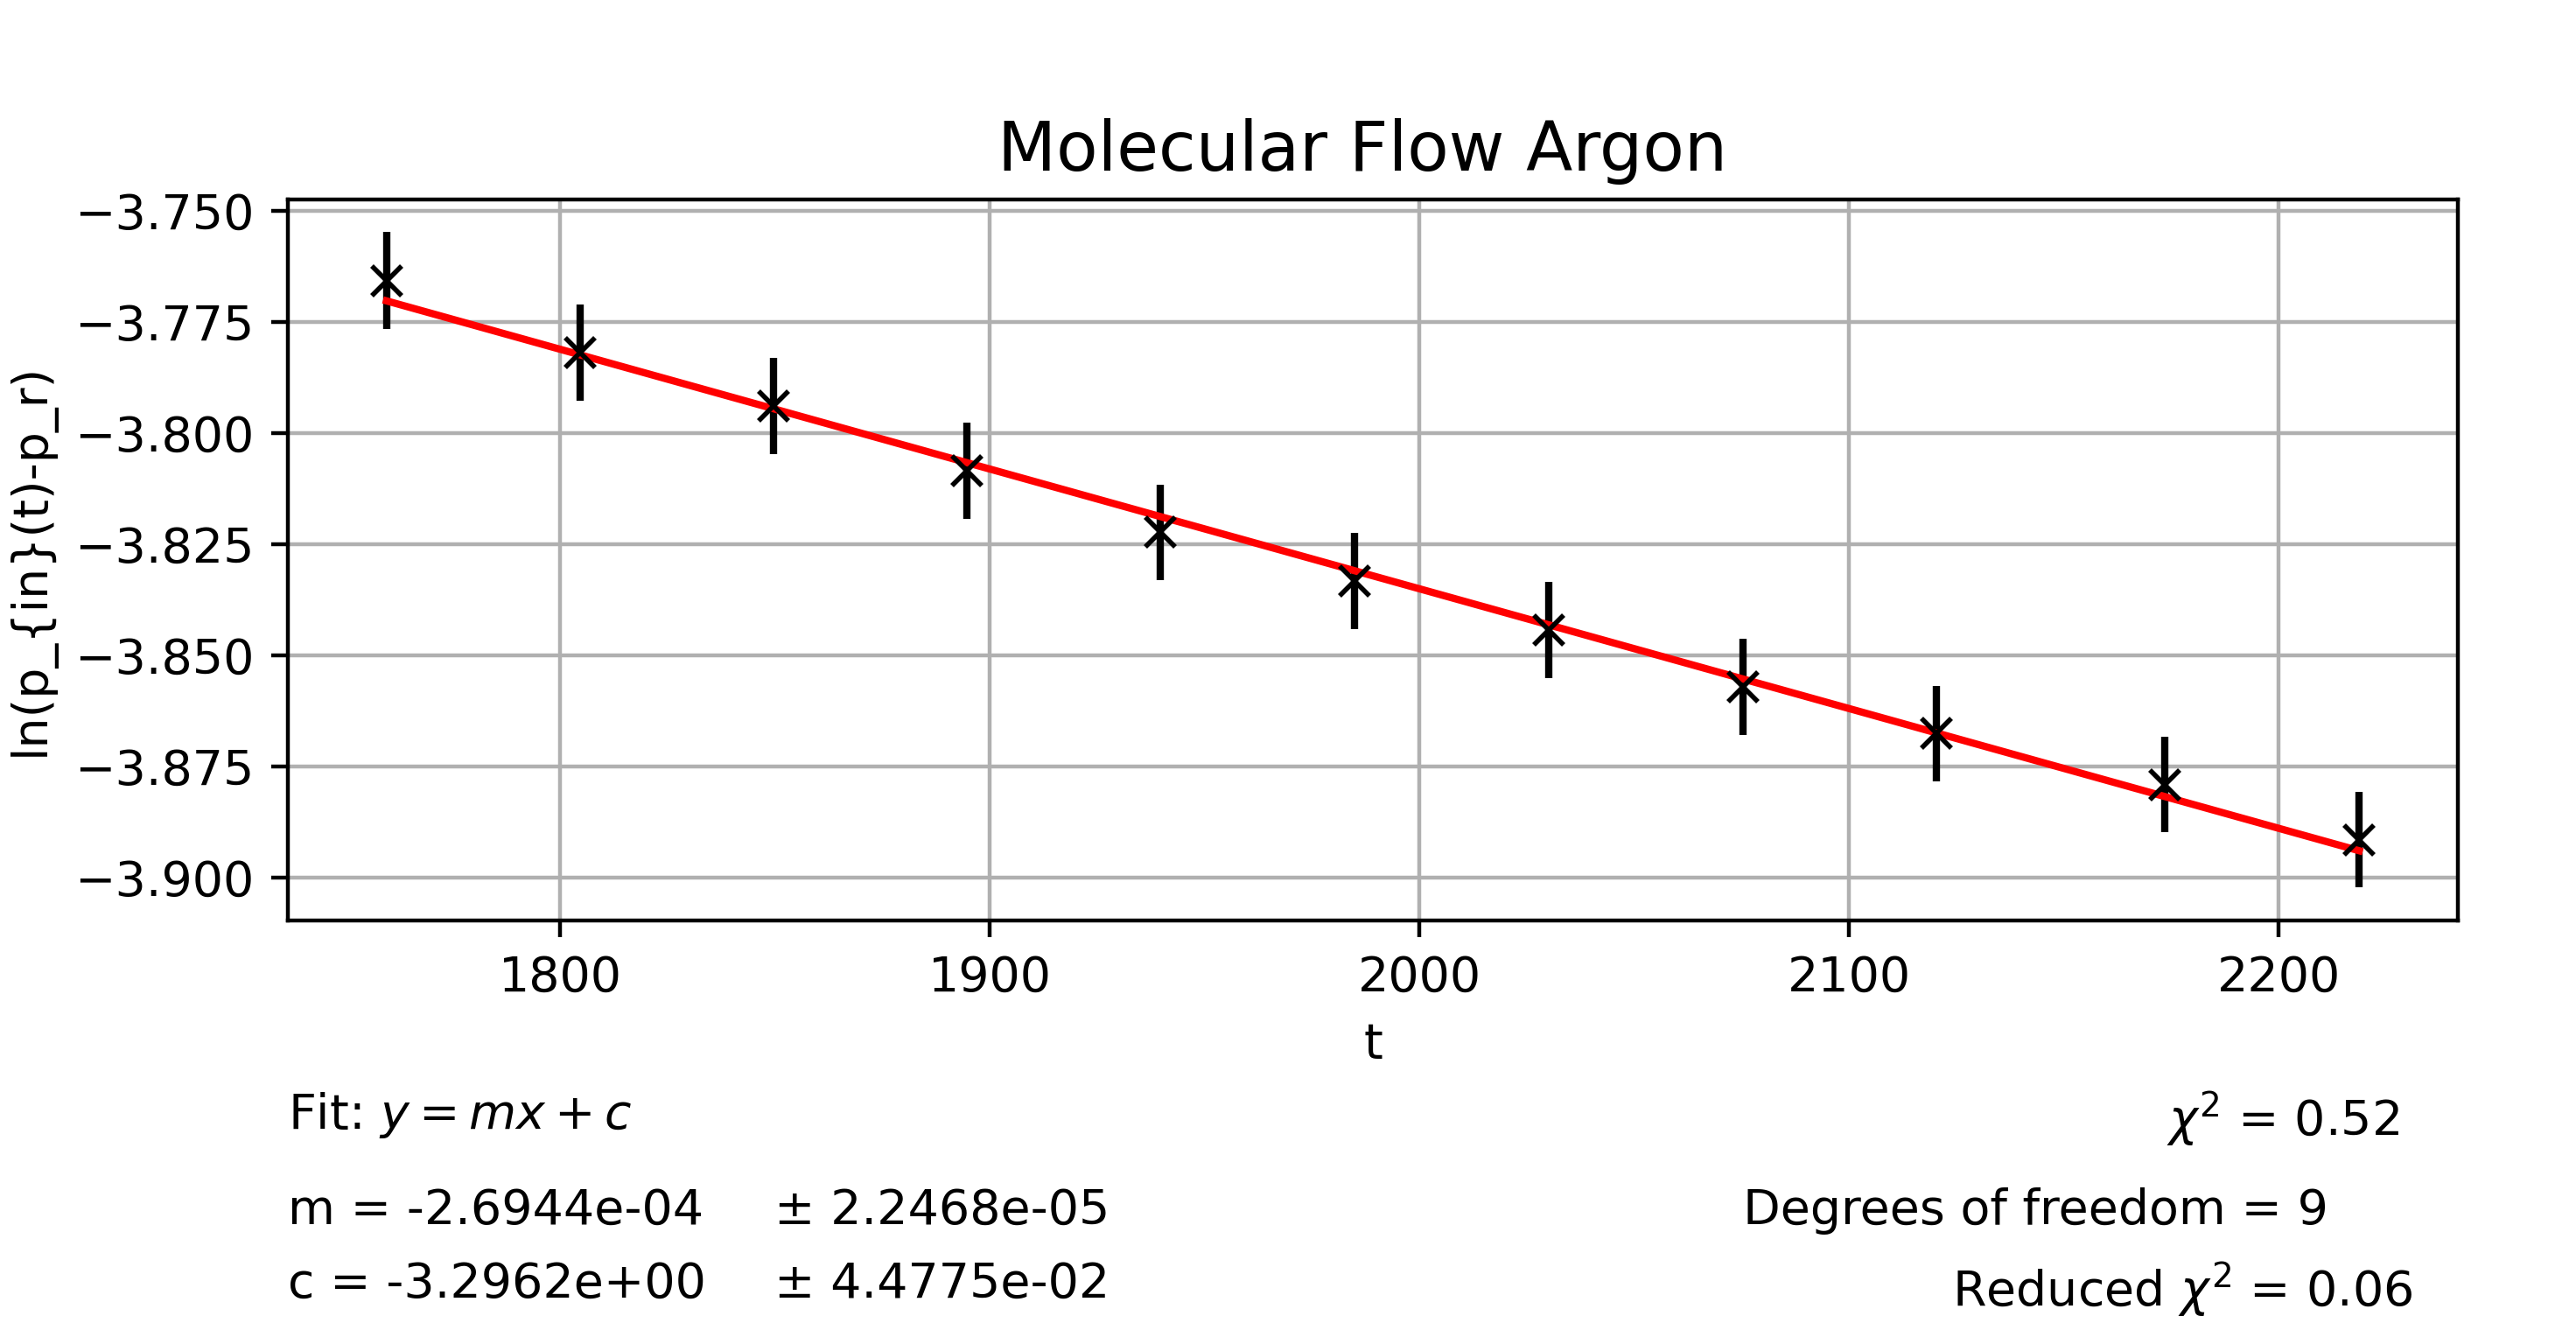
\includegraphics[scale=0.5]{Molecular_Argon.png}
		\caption{This graph shows the best-fit line of our data. The gradient of the best fit line is $-2.69 \times 10^{-4} \pm 2.2 \times 10^{-5}$}
		\end{center}
	\end{figure}
	
	Following a similar reasoning, we reckon the pumping speed of Ar is
	\begin{equation}
		S_{Ar}= 2 \pm 10 \si{\meter^3\per\second}.
	\end{equation}
	\section{Discussion}
	\subsection{Laminar Flow}
	In the laminar flow experiment, our result is not precise. The uncertainty of the viscosity is large. It has a magnitude of about $10^{-2}$, whereas the reference value of the viscosity of both gases at $20\si{\celsius}$ is about a magnitude of $10^{-5}$.
	
	Now, we try to analyse factors contributing to the uncertainty of $\eta$. Five factors ($a^4$, $p_{out}$, $m$, $V_{in}$, and $l$) contributed to the uncertainty of viscosity. $\sigma_{a^4}=1 \times 10^{-17}$, $\sigma_{p_{out}}=256$, $\sigma_{V_{in}}=0.006$, $\sigma_{l}=5 \times 10^{-4}$, and $\sigma_{m}=6.83 \times 10^{-4}$. $\sigma_{p_{out}}$ made for most of the uncertainty in viscosity. This is due to the intrinsic resolution of PT 1, which has an uncertainty of $2.5\%$. Therefore, a possible way of improving the precision of the result is to use a gauge with more accuracy.
	
	Assuming the actual measure lies in the centre. of our error bar, our data is fairly accurate. At $20\si{\celsius}$, the reference value for $\eta_{He}$ is $1.96 \times 10^{-5}. \si{\newton\cdot\second\per\metre^2}$, and for $\eta_{Ar}$ is $2.23 \times 10^{-5} \si{\newton\cdot\second\per\metre^2}$ 
	
	\subsection{Molecular Flow}
	Similar problems with uncertainty appeared in the estimation of pumping speed. The input volume is the major contributing factor to the uncertainty of pumping speed. This, however, is also linked to the resolution of the pressure gauge, because we computed the input volume using the ideal gas law, which involves pressure.	
	
	Also, if assuming the actual value of our measurement lies in the centre of the error bar, our estimation is fairly accurate. The theoretical value of $S_{He}$ is $2.6\si{\meter^3\per\second}$, and $S_{Ar}$ is $8.6\si{\meter^3\per\second}$.\cite{Viscosity}
	 
	
	
\printbibliography
	



\end{document}
